\documentclass[11pt, a4paper]{article}

\usepackage[utf8]{inputenc}
\usepackage[T1]{fontenc}
\usepackage[english]{babel}

\usepackage{amsmath}
\usepackage{graphicx}
\usepackage{float}%option [H] for floats.

\title{INFOH414 -- Swarm Intelligence: Collective Decision Making with Homogeneous Agents}
\author{Quentin Delhaye}
\date{}

\begin{document}
\maketitle


\section{Introduction}
The aim of this project is for a homogeneous group of robots to take a collective decision.
In this case, the decision is to decide on the highest quality room and to converge to it.
Tha quality of a room is defined by two attributes: the ground colour $v_g$ and the number of objects in the room $v_o$.
Their average yields the quality $v$ of a room: \[v = \frac{(v_g + v_o)}{2}\]

Each robot is fully capable of sensing the quality of a room on its own, but its limited memory allows it to remember only one at a time.

The trick is to disperse the robots in the arena, exchange information when they come back in the central room to finaly converge to the same, highest quality room.









\section{Robot behaviour}
The basic idea is to have each robot move around and calculate the quality of each room.
After moving for a while in the room, they go back to the central room and broadcast their quality using LEDs and sense other's beacons at the same time.
They then move to the highest quality room broadcasted in the central room


The following description dives more into the details of its behaviour, as does the figures \ref{fig:state-machine} and \ref{fig:activity}.

\begin{enumerate}
	\item The robot starts in the central room
	\item Find the closest room using the omnidirectional camera and move toward it.
	\item Near the entrace of the room, there is an ``inhibition" circle. Upon entering that area, the robot does no longer care for the obstacles and runs straight forward through the entrance until it leaves the circle again
	\item The robot is now considered to be in the room. It senses the quality of the room and wanders in there for \texttt{STEPS\_UNTIL\_LEAVE} steps.
	\item After that, it heads back to the room entrance.
	\item Once back in the central room, it broadcasts the room quality as well as the room number.
	\item At the same time, it reads the quality broadcasted by the others. If it's higher than its, it sets that room as its new target room. Otherwise, it keeps its old room as the target.
	\item During that time, it continues to wander in the central room for\newline{} \texttt{MAX\_CENTRAL\_ROOM\_WANDER\_STEPS} steps.
	\item After that, it heads to its target room. If everything went according to plan, it had enough time to have a taste of all the rooms from the other robots and is now heading for the highest quality room.
	\item Knowing that, it enters the room and stays there for\newline{} \texttt{STEPS\_UNTIL\_LEAVE\_BEST\_ROOM} steps, before begining the same cycle over and over again.
\end{enumerate}

The quality of the room is broadcasted according to the following encoding:
\begin{itemize}
	\item Red component = $(\mbox{room number} + 1) * 40$
	\item Green component = $42$
	\item Blue component = $(\mbox{quality}*200)+20$
\end{itemize}
Only the beacon LED is lit.



~\newline{}
Please note that on top of the best room determination, the obstacle avoidance algorithm also runs.
This specific piece of code is a slightly adapted version from the first practical exercices ``\texttt{obstacleAvoidance\_sta.lua}".


\begin{figure}[H]
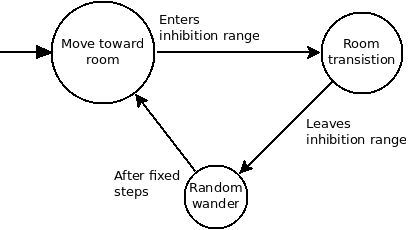
\includegraphics[width=.95\textwidth]{state-machine}
\caption{State machine of the robot}
\label{fig:state-machine}
\end{figure}

\begin{figure}[H]
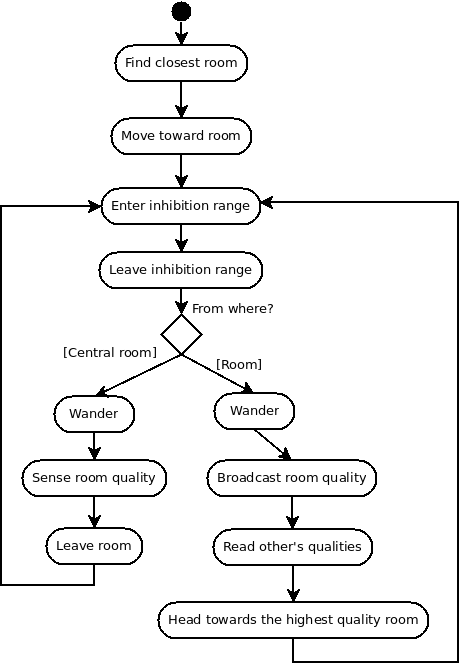
\includegraphics[width=.95\textwidth]{activity}
\caption{Activity diagram of a typical execution}
\label{fig:activity}
\end{figure}





\section{Results}
The controller is not able to produce consistent results\footnote{Meaning it fails miserably on numerous simulations.}.

Using 20 robots, it takes around 2380 steps to have 90\% of the population in the highest quality room.
At this point, the congestion at the room entrance is already pretty high and a better management on this regard could reduce the necessary steps by 500 to 700.

With 30 robots, the simulation struggles to get up to 50\% agglomeration in the same number of steps as with 20 robots.
90\% Could not be reached because of the engorgement at the room entrance.

With 40 robots, it takes almost twice the time to get those 50\%
~\\

Knowing that using more robots worsens the situation, the simulation was tested with less of them, which should yield better results.
The result coroborates the assumption as less than 1700 steps were needed to reach 80\% convergence with 10 robots.
The 90\% goal is way harder to reach as only one robot is allowed to failed with the objective in this configuration.

\section{Conclusion}
Many improvements can be made to this project, especially to the congestion problem.

\begin{itemize}
	\item The collision between the robots is poorly handled.
	It often happen that robots block each others at the entrace of the rooms.
	In this particular case, a circulation routing would be a better implementation; the robots could keep right by keeping the room beacon on their left, for example.
	\item The ``random wadering" is not so random. Currently, it relies on the collision avoidance change the trajectory of the robot.
	\item The inhibition circle is not an ideal solution. The robots are forcing they way through the entrance when it would be smarter to set a priority scheme.
	\item Robots should stay longer in a room if there are many other robots with them. With the current implementation, they want to leave after a fixed number of steps. However, the larger the swarm, the more difficult it is to have them all in one room at the same time.
\end{itemize}

\end{document}
